\documentclass[12pt, twoside]{book}
%\documentclass[12pt, oneside]{book}  % jednostranna tlac

%spravne nastavenie okrajov
\usepackage[a4paper,top=2.5cm,bottom=2.5cm,left=3.5cm,right=2cm]{geometry}
%zapnutie fontov pre UTF8 kodovanie
\usepackage[utf8]{inputenc}
\usepackage[T1]{fontenc}

%zapnutie slovenskeho delenia slov
%a automatickych nadpisov ako Obsah, Obrázok a pod. v slovencine
\usepackage[slovak]{babel} % vypnite pre prace v anglictine!

%nastavenie riadkovania podla smernice
\linespread{1.25} % hodnota 1.25 by mala zodpovedat 1.5 riadkovaniu

% balicek na vkladanie zdrojoveho kodu
\usepackage{listings}

% nastavenia balicka listings
\renewcommand{\lstlistingname}{Algoritmus}
\lstset{extendedchars=true, basicstyle=\small, frame=lines,
    commentstyle=\color{olive}\textit, keywordstyle=[1]\color{blue},
    literate=
    {á}{{\'a}}1 {ä}{{\"a}}1 {č}{{\v{c}}}1 {ď}{{\v{d}}}1 {é}{{\'e}}1 {í}{{\'i}}1
    {ĺ}{{\'l}}1 {ľ}{{\v{l}}}1 {ň}{{\v{n}}}1 {ó}{{\'o}}1 {ô}{{\^o}}1 {š}{{\v{s}}}1
    {ť}{{\v{t}}}1 {ú}{{\'u}}1 {ý}{{\'y}}1 {ž}{{\v{z}}}1
    {Á}{{\'A}}1 {Č}{{\v{C}}}1 {Ď}{{\v{D}}}1 {É}{{\'E}}1 {Í}{{\'I}}1 {Ĺ}{{\'L}}1 
    {Ľ}{{\v{L}}}1 {Ň}{{\v{N}}}1 {Ó}{{\'O}}1 {Š}{{\v{S}}}1 {Ť}{{\v{T}}}1 {Ú}{{\'U}}1
    {Ý}{{\'Y}}1 {Ž}{{\v{Z}}}1
}
\lstdefinelanguage{AVR}{
    keywords={clr, eor, cpi, breq, inc, tst, brne, ldi, nop, add, sub, mov, or, dec, ldr, str},
    sensitive=false,
    comment=[l]{;},
}

% balicek na vkladanie obrazkov
\usepackage{graphicx}
\usepackage{subfig}
% balicek na vkladanie celych pdf dokumentov
\usepackage{pdfpages}
% balicek na vkladanie diagramov
\usepackage{pgfplots}
\pgfplotsset{width=0.6\textwidth,compat=1.9}
% balicek na spravne formatovanie URL
\usepackage{url}
% balicek na hyperlinky v ramci dokumentu
% zrusime farebne ramiky okolo liniek
\usepackage[hidelinks,breaklinks]{hyperref}



% -------------------
% --- Definicia zakladnych pojmov
% --- Vyplnte podla vasho zadania, rok ma byt rok odovzdania
% -------------------
\def\mfrok{2023}
\def\mfnazov{Útoky na hardvér\\pomocou indukovania chýb}
\def\mftyp{Bakalárska práca}
\def\mfautor{Dennis Vita}
\def\mfskolitel{RNDr. Richard Ostertág, PhD. }

%ak mate konzultanta, odkomentujte aj jeho meno na titulnom liste
\def\mfkonzultant{tit. Meno Priezvisko, tit. }  

\def\mfmiesto{Bratislava, \mfrok}

\def\mfodbor{ Informatika}
\def\program{ Informatika }


% Ak je školiteľ z FMFI, uvádzate katedru školiteľa, zrejme by mala byť aj na zadaní z AIS2
% Ak máte externého školiteľa, uvádzajte Katedru informatiky 
\def\mfpracovisko{ FMFI.KI - Katedra informatiky }

\begin{document}     
\frontmatter
\pagestyle{empty}

% -------------------
% --- Obalka ------
% -------------------

\begin{center}
\sc\large
Univerzita Komenského v Bratislave\\
Fakulta matematiky, fyziky a informatiky

\vfill

{\LARGE\mfnazov}\\
\mftyp
\end{center}

\vfill

{\sc\large 
\noindent \mfrok\\
\mfautor
}

\cleardoublepage
% --- koniec obalky ----

% -------------------
% --- Titulný list
% -------------------


\noindent

\begin{center}
\sc  
\large
Univerzita Komenského v Bratislave\\
Fakulta matematiky, fyziky a informatiky

\vfill

{\LARGE\mfnazov}\\
\mftyp
\end{center}

\vfill

\noindent
\begin{tabular}{ll}
Študijný program: & \program \\
Študijný odbor: & \mfodbor \\
Školiace pracovisko: & \mfpracovisko \\
Školiteľ: & \mfskolitel \\
% Konzultant: & \mfkonzultant \\
\end{tabular}

\vfill


\noindent \mfmiesto\\
\mfautor

\cleardoublepage
% --- Koniec titulnej strany


% -------------------
% --- Zadanie z AIS
% -------------------
% v tlačenej verzii s podpismi zainteresovaných osôb.
% v elektronickej verzii sa zverejňuje zadanie bez podpisov
% v pracach v angličtine anglické aj slovenské zadanie

\newpage 
\setcounter{page}{2}
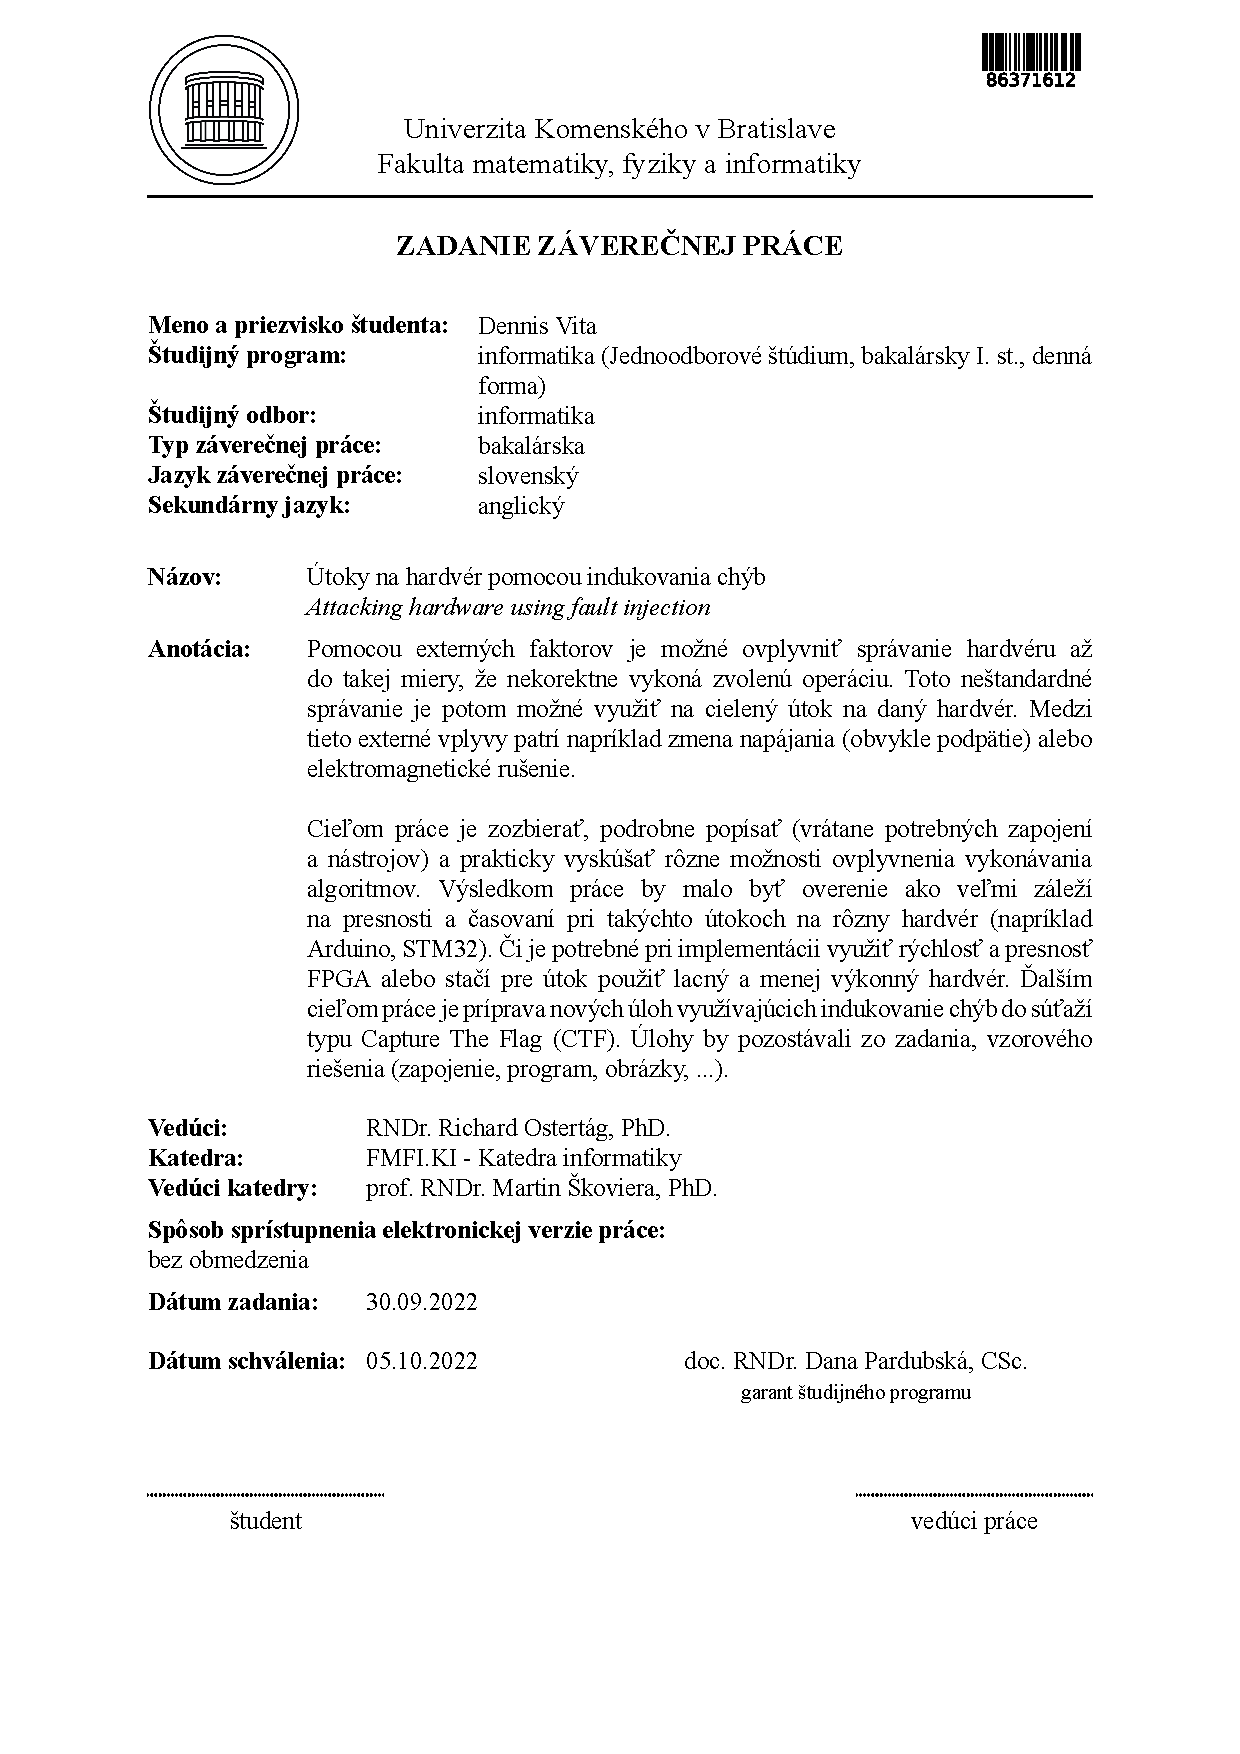
\includepdf{images/zadanie.pdf}

% --- Koniec zadania


% -------------------
%   Poďakovanie - nepovinné
% -------------------
\newpage 
\pagestyle{plain}
~

\vfill
{\bf Poďakovanie:} Ďakujem vedúcemu bakalárskej práce RNDr. Richardovi Ostertágovi, PhD. za odborné pripomienky a rady k ...[Dokončiť]

% --- Koniec poďakovania

% -------------------
%   Abstrakt - Slovensky
% -------------------
\newpage 
\section*{Abstrakt}

Vplyvom externých fyzikálnych faktorov (zmena napájania, elektromagnetické rušenie a pod.) je možné ovplyvniť činnosť hardvéru až do takej miery, že nekorektne vykoná niektorú operáciu. Indukovanie chýb je technika útoku, ktorá zneužíva toto správanie a možno pomocou nej cielene zaútočiť na konkrétny hardvér. Pri správnom načasovaní na konkrétnu časť programu je možné cielene ovplyvniť daný hardvér, napríklad s účelom obísť bezpečnostný mechanizmus alebo narušiť implementáciu kryptografického algoritmu. Cieľom práce je overiť, či aj lacným hardvérom možno realizovať úspešný útok. Zároveň sa v práci zaoberáme podrobnou analýzou vybraných útokov a ich možným dopadom na konkrétny hardvér (mikrokontrolér ATMega328P). Cieľom je aj zistiť aké možnosti pre útočníka lacný hardvér poskytuje. Výsledky analýzy na záver demonštrujeme úspešnými útokmi na jednoduché príklady programov.

\paragraph*{Kľúčové slová:} indukovanie chýb, mikrokontrolér, zmena napájania
% --- Koniec Abstrakt - Slovensky


% -------------------
% --- Abstrakt - Anglicky 
% -------------------
\newpage 
\section*{Abstract}

The influence of external physical factors (power supply changes, electromagnetic interference, etc.) can affect the operation of hardware to such an extent that it may incorrectly execute an operation. Fault injection is an attack technique that exploits this behavior and can be used to attack specific hardware. By proper timing and targeting a specific part of a program, it is possible to deliberately influence the targeted hardware, for example, to bypass a security mechanism or cause faults in an implementation of a cryptographic algorithm. The goal of this thesis is to verify whether successful attacks can also be performed using inexpensive hardware. Additionally, the thesis focuses on a detailed analysis of selected attacks and their potential impact on specific hardware (the ATMega328P microcontroller). The aim is also to explore what capabilities inexpensive hardware to an attacker provides. The analysis results are demonstrated by successful attacks on simple program examples.


\paragraph*{Keywords:} fault injection, microcontroller, power glitch

% --- Koniec Abstrakt - Anglicky

% -------------------
% --- Predhovor - v informatike sa zvacsa nepouziva
% -------------------
%\newpage 
%
%\chapter*{Predhovor}
%
%Predhovor je všeobecná informácia o práci, obsahuje hlavnú charakteristiku práce 
%a okolnosti jej vzniku. Autor zdôvodní výber témy, stručne informuje o cieľoch 
%a význame práce, spomenie domáci a zahraničný kontext, komu je práca určená, 
%použité metódy, stav poznania; autor stručne charakterizuje svoj prístup a svoje 
%hľadisko. 
%
% --- Koniec Predhovor


% -------------------
% --- Obsah
% -------------------

\newpage 

\tableofcontents

% ---  Koniec Obsahu

% -------------------
% --- Zoznamy tabuliek, obrázkov - nepovinne
% -------------------

\newpage 

\listoffigures
\listoftables

% ---  Koniec Zoznamov

\mainmatter
\pagestyle{headings}


\input 00-uvod.tex 

\input 01-teoria.tex

\input 02-hardver.tex

\input 03-utoky.tex

\input 04-CTF.tex

\input 05-zaver.tex

% -------------------
% --- Bibliografia
% -------------------


\newpage	

\backmatter

\thispagestyle{empty}
\clearpage

\bibliographystyle{plain}
\bibliography{literatura} 

%Prípadne môžete napísať literatúru priamo tu
%\begin{thebibliography}{5}
 
%\bibitem{br1} MOLINA H. G. - ULLMAN J. D. - WIDOM J., 2002, Database Systems, Upper Saddle River : Prentice-Hall, 2002, 1119 s., Pearson International edition, 0-13-098043-9

%\bibitem{br2} MOLINA H. G. - ULLMAN J. D. - WIDOM J., 2000 , Databasse System implementation, New Jersey : Prentice-Hall, 2000, 653s., ???

%\bibitem{br3} ULLMAN J. D. - WIDOM J., 1997, A First Course in Database Systems, New Jersey : Prentice-Hall, 1997, 470s., 

%\bibitem{br4} PREFUSE, 2007, The Prefuse visualization toolkit,  [online] Dostupné na internete: <http://prefuse.org/>

%\bibitem{br5} PREFUSE Forum, Sourceforge - Prefuse Forum,  [online] Dostupné na internete: <http://sourceforge.net/projects/prefuse/>

%\end{thebibliography}

%---koniec Referencii

% -------------------
%--- Prilohy---
% -------------------

%Nepovinná časť prílohy obsahuje materiály, ktoré neboli zaradené priamo  do textu. Každá príloha sa začína na novej strane.
%Zoznam príloh je súčasťou obsahu.
%
\input 06-prilohaCD.tex

\end{document}